\documentclass[12pt]{article}
\usepackage{preamble}

\pagestyle{fancy}
\fancyhead[LO,LE]{Теория вероятности}
\fancyhead[CO,CE]{03.09.2024}
\fancyhead[RO,RE]{Лекции Блаженова А. В.}

\fancyfoot[L]{\scriptsize исходники найдутся тут: \\ \url{https://github.com/pelmesh619/itmo_conspects} \Cat}

\begin{document}
    В теории вероятности обычно изучают случайные события

    Обычно наука занимается закономерностями, но так как в случайных экспериментах нет закономерностей, теория
    вероятности занимается поисков закономерности в сериях случайных экспериментах

    Итак, в XVI веке начали с экспериментов бросков монеты:

    \begin{tabular}{ccc}
        число бросков & число гербов & частота \\
        4040 & 2048 & 0.5069 \\
        12000 & 6019 & 0.5016 \\
        24000 & 12012 & 0.5005 \\
    \end{tabular}

    Как можно видеть, частота стремится к 0.5 - появляется статистическая закономерность

    \section{1. Статистическое определение вероятности}

    Пусть проводится $n$ реальных экспериментов, при которых событие $A$ появилось $n_A$ раз

    Отношение $\frac{n_A}{n}$ называется частотой события $A$

    Эксперименты показывают, что при увеличении числа $n$ частота стабилизируется у некоторого числа,
    при котором мы понимаем статистическую вероятность: $P(A) \approx \frac{n_A}{n}$ при $n \to \infty$

    \subsection{Пространство элементарных исходов. Случайные события}

    \Def Пространством элементарных исходов $\Omega$ называется множество, содержащее все возможные исходы
    экспериментов, из которых при испытании происходит ровно один. Элементы этого множества называются
    элементарными исходами и обозначаются $\omega$

    \Def Случайными событиями называется подмножество $A \subset \Omega$. События $A$ наступают, если произошел один из
    элементарных исходов из множества $A$

    \ExN{1} Бросок монеты: $\Omega = \{\text{Г}, \text{Р}\}$, $A = \{\text{Г}\}$ - выпал герб

    \ExN{2} Игральная кость: $\Omega = \{1, 2, 3, 4, 5, 6\}$, $A = \{\text{выпало четное число}\} = \{2, 4, 6\}$

    \ExN{3} Монета бросается дважды.

    a) Учитываем порядок: $\Omega = \{\text{ГГ}, \text{РР}, \text{РГ}, \text{ГР}\}$

    a) Не учитываем порядок: $\Omega = \{\text{ГГ}, \text{РР}, \text{ГР}\}$

    \ExN{4} Кубик дважды: $\Omega = \{\Pair{i, j} \ | \ 1 \leq i, j \leq 6\}$

    $A = \{\text{разность} \ \vdots \ 3\} = \{\Pair{1, 4}; \Pair{4, 1}; \Pair{2, 5}; \Pair{5, 2}; \dots\}$

    \ExN{5} Монета бросается до первого герба: $\Omega = \{\text{Г}, \text{РГ}, \text{РРГ}, \dots\}$ - счетно-бесконечное множество

    \ExN{6} Монета бросается на плоскость: $\Omega = \{\Pair{x, y} \ | \ x, y \in \Real, \Pair{x, y} \text{ - центр монеты}\}$ - несчетное число исходов

    \sebsection{Операции над событиями}

    $\Omega$ - достоверные события (наступают всегда)

    $\emptyset$ - невозможное события (никогда не наступает, так как не содержит ни одного элем. исхода)

    Введем операции:

    \DefN{1} Суммой $A + B$ называется событие, состоящее в том, что произошло события $A$ или событие $B$ (хотя бы одно из них)

    \DefN{2} Произведением $A \cdot B$ называется событие, состоящее в том, что произошло событие $A$ и событие $B$ (оба из них)

    \Notas $A_1 + A_2 + \dots + A_n + \dots$ - произошло хотя бы одно из этих событий

    $A_1 \cdot A_2 \cdot \dots \cdot A_n \cdot \dots$ - произошли все эти события

    \DefN{3} Противоположным $A$ событием называется событие $\overline{A}$, состоящее в том, что событие $A$ не произошло

    \Notas $\overline{A} = A$ % не понял почему

    \DefN{4} Дополнение (разность) $A \setminus B$ называется событие $A \cdot \overline{B}$

    \DefN{5} События $A$ и $B$ называются несовместными, если их произведение - пустое множество
    (не могут произойти одновременно при одной эксперименте)

    \DefN{6} События $A$ влечет события $B$, если $A \subset B$ (если наступает $A$, то наступит $B$)

    \subsection{Вероятность}

    Мы хотим присвоить какую-то числовую характеристику к каждому событию,
    отражающее его частоту наступления: $0 \leq P(A) \leq 1$ - вероятность наступления события $A$

    \mediumvspace

    \textbf{Классическое определение вероятности}

    Пусть пространство случайных событий $\Omega$ содержит конечное число равновозможных исходов,
    тогда применимо классическое определение вероятности

    \Def \fbox{$P(A) = \frac{|A|}{|\Omega|} = \frac{m}{n}$}, где $n$ - число всех возможных исходов, $m$ - число благоприятных исходов

    В частности, если $\Omega = n$ и $A_i$ - элем. исх., то $P(A_i) = \frac{1}{n}$

    Свойства:

    1) $0 \leq P(A) \leq 1$

    2) $P(A) = 1 \quad (m = n)$

    3) $P(\emptyset) = 0 \quad (m = 0)$

    4) Если события $A$ и $B$ несовместны, то $P(A + B) = P(A) + P(B)$

    \mediumvspace

    \textbf{Геометрическое определение вероятности (граф де Бюффон)}

    Пусть $\Omega \subset \Real^n$ - замкнутая ограниченная область

    $\mu(\Omega)$ - мера $\Omega$ в $\Real^n$ (например, длина отрезка, площадь области на плоскости, объем тела в пространстве)

    В эту область наугад бросаем точку. \enquote{Наугад} означает, что вероятность попадания в $A$ зависит только от меры $A$ и не зависит от ее расположения

    В этом случае применимо геометрическое определение вероятности

    $P(A) = \frac{\mu(A)}{\mu(\Omega)}$

    \ExN{1} Монета диаметром в 6 см бросается на пол, вымощенной квадратной плиткой со стороной 20 см, какова вероятность,
    что монета окажется целиком внутри одной плитки

    $\mu(\Omega) = 20^2 = 400$

    $\mu(A) = (20 - 3 - 3)^2 = 196$

    $P(A) = \frac{\mu(A)}{\mu(\Omega)} = \frac{196}{400} = 0.49$

    \hypertarget{buffonsproblem}{}

    \ExN{2} Задача Бюффона об игле: пусть пол вымощен ламинатом, $2l$ - ширина доски, на пол бросается игла длины, равной ширине доски,
    найти вероятность того, что игла пересечет стык доски

    \smallvspace

    \begin{minipage}{\linewidth}
        \begin{wrapfigure}{r}{0pt}
            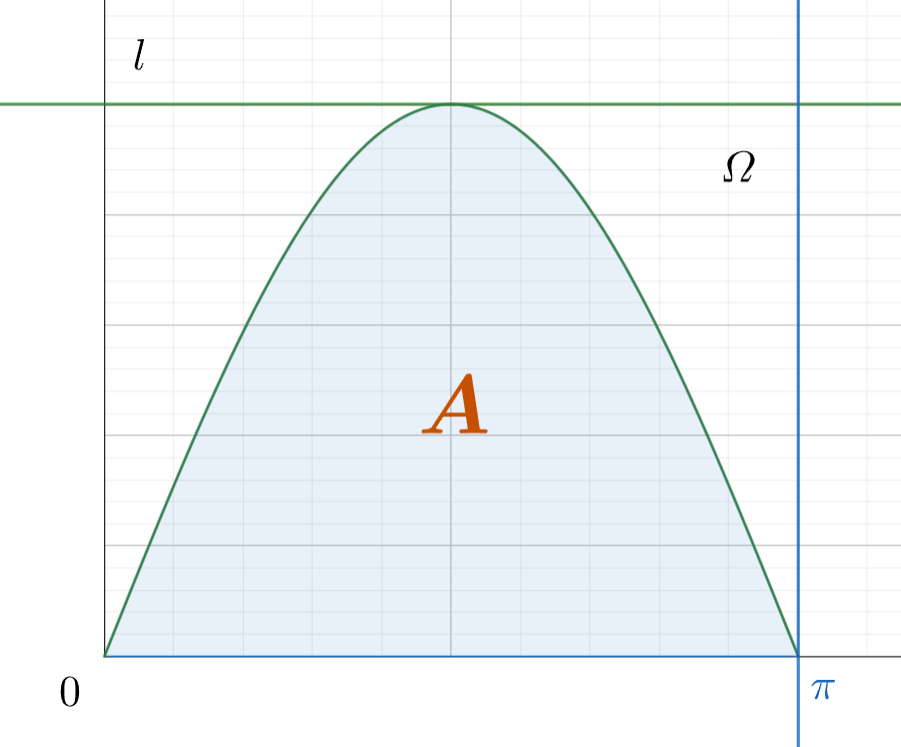
\includegraphics[height=6cm]{probtheory/images/probtheory_2024_09_03_1}
        \end{wrapfigure}

        Определим положение иглы координатами центра и углом, между иглой и стыком доски, причем можно считать, что эти величины независимы

        $\letsymbol x \in [0; 1]$ - расстояние от центра до ближайшего края, $\varphi \in [0; \pi]$ - угол

        $\Omega = [0; 1] \times [0; \pi]$

        Событие $A$ (пересечет стык) наступает, если $x \leq l \sin \varphi$

        $P(A) = \frac{S(A)}{S(\Omega)}$

        $S(\Omega) = \pi l$

        $S(A) = \int_0^\pi l \sin \varphi d\varphi = -l \cos \varphi \Big|_0^\pi = -l (-1 - 1) = 2l$

        $P(A) = \frac{2l}{\pi l} = \frac{2}{\pi}$
    \end{minipage}
\end{document}
